\section{Experiments }
\label{sec:exp}

The benchmark data sets used are the commonly known data sets: the road network of Aalborg\footnote{http://www.dbxr.org/experimental-guidelines/}, Beijing\footnote{http://arxiv.org/abs/cs/04100001}
and Singapore \citep{Song2014PRESS}. All data sets consist of a large number of nodes, edges, and associated weights. Table \ref{tab:datasetinfo} summarizes the information on the data sets.

 \begin{table}[h]
 \caption{Information of data sets.}
 \centering
 \label{tab:datasetinfo}
{
 \begin{tabular}{|c|c|c|c|}
 \hline
  Data set   & Number of nodes &Number of edges & Description\\
  \hline
  Aalborg    &3.9Million&4.6Million&Road network\\
  \hline
   Beijing   &2.4Million&2.7Million&Road network\\
  \hline
   Singapore & 20,800&55,890&Road network\\
   \hline
 \end{tabular}
}
\end{table}

We divide each data set into two parts: one part for training and the other part for testing. Training sets act as historical logs while test sets act as future queries. The frequency statistics are extracted from the training set, and the cache is filled based on benefit values.
For Aalborg, there are 2673 and 2573 queries in training and test sets, respectively; for Beijing, there are 7177 and 6664 queries in training and test sets, respectively; for Singapore, we draw 20,000 queries from a long-tail distribution, which is close to the practical situation. Out of the 20,000 queries, 70\% queries are seen as the training set and remnant 30\% queries as the test set.

To simulate the weight change of an edge, we generate 50 instances based on each data set. In each instance, one edge is randomly selected and its weight is changed. Out of the 50 instances, 20 instances increase weights of edges and 30 instances decrease weights of edges.
The increase and decrease of weights range from 1\% to 100\%.


We assume that the query trend on training sets and test sets are similar, and the statistic information from training sets can predict future queries to some extent. All the code was implemented in GNU C++. The experiments were run on a PC with an Intel i7 Quad Core CPU clocked at 3.10 GHz.

\subsection{Effect of Cache Structure}
\label{sec:effect-cache-structure}
We use a bitmap-based structure in Section~\ref{sec:Cache Structure} to facilitate the cache on answering users' queries.
To have an impression of how the bitmap structure works, we compare it with a benchmark structure, which only records shortest paths in a path array.
Queries are answered by scanning the array.
The benchmark structure is called a basic cache.

For each data set, the cache is firstly initialized based on the largest benefit values of paths in the query log. Queries in the test sets arrive one by one and the total response time by two cache structure is displayed in Figure~\ref{fig:time-cache-structure}. We can see that the time performance of bitmap structure is much better than that of basic structure. The response time of bitmap is only 0.7ms when the cache size is 9MB for the Aalborg data set, while it costs 205ms for the basic structure. We can get consistent results on Beijing and Singapore data sets.
Moreover, the response time is almost constant with the increase of cache size for the bitmap structure.
\begin{figure}[htbp]
\centering
    \subfigure[{\footnotesize Aalborg}]
   {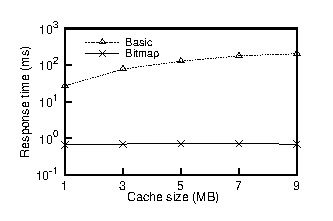
\includegraphics
   [height=3.5cm]{figure/construct-cache-time-aal.eps}}
   \subfigure[{\footnotesize Beijing}]
   {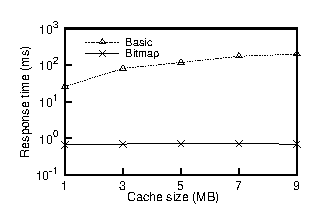
\includegraphics [height=3.5cm]{figure/construct-cache-time-beijing.eps}}
   \subfigure[{\footnotesize Singapore}]
   {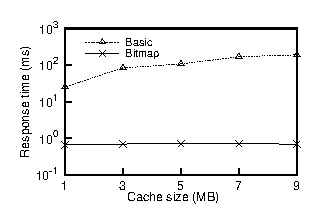
\includegraphics [height=3.5cm]{figure/construct-cache-time-singapore.eps}}
 \caption{Response time of cache structures.}
 \label{fig:time-cache-structure}
\end{figure}


\subsection{Efficiency of Detecting Affected Paths in the Cache}
\label{ssec:efficiency-detecting}
Detecting affected paths in a cache is an important step before refreshing a cache. To demonstrate the performance of our algorithms, a naive method (NM) is used as a benchmark method. Due to the size of graph, NM only re-computes new shortest paths for all pairs of nodes in the cache and compares them with the original ones. If the two shortest paths for a pair of nodes are different, then an affected path is detected.
We test our three affected paths detecting algorithms NEA, ONE, INE and NM on Aalborg, Beijing and Singapore data sets and the detection time of the four detection methods is regarded as the performance indicator.

The experimental result on each data set is the average of 50 instances.
As seen from Figure~\ref{fig:comparison-detecttime}, all of our algorithms have a better performance than NM.
For example, in the Aalborg data set, when the cache size is 9MB, the algorithm INE achieves the best time performance and its detection time is only 131ms, while NM costs 28.67s. Meanwhile, we observe that INE is slightly superior to ONE and ONE is superior to NEA. This is consistent with our expectation.
\begin{figure}[htbp]
\centering
   \subfigure[{\footnotesize Aalborg}]
   {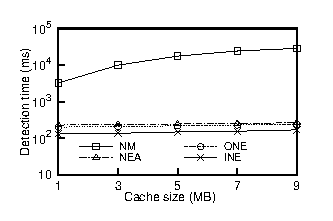
\includegraphics
   [height=3.5cm]{figure/A-size-time.eps}}
   \subfigure[{\footnotesize Beijing}]
   {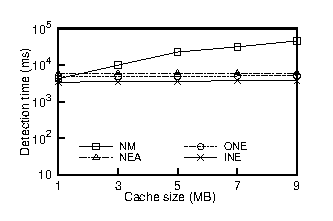
\includegraphics [height=3.5cm]{figure/A-size-time-beijing.eps}}
   \subfigure[{\footnotesize Singapore}]
   {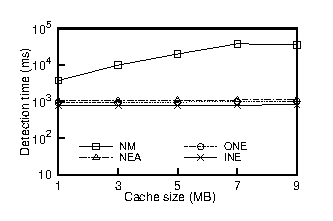
\includegraphics [height=3.5cm]{figure/singapore-detectaffect-time.eps}}
 \caption{Performance of affected path detection methods.}
 \label{fig:comparison-detecttime}
\end{figure}

%In addition, we can see the detection time is generally proportional to the size of graph.
%Aalborg has minimal time cost, Singapore has mediate time cost, and Beijing has the most time cost. The graph of Aalborg is sparse, the graph of Singapore is intermediate, and Beijing is dense. The denser a graph is, the more time it will cost because the algorithms check more paths in a dense graph to yield affected paths.

\subsection{Performance of Refreshment Strategies}
\label{ssec:overhead-strategy}
For ease of illustration, reloading the whole cache, replacing affected paths with the largest benefit values, replacing affected paths with the highest frequency paths and replacing affected paths using roulette wheel selection are abbreviated as RWC, RLB, RHF and RRWS, respectively.

Figure~\ref{fig:comparison-hit} shows the hit-ratios of four refreshment strategies under different scales of caches.
We sum up hit ratio of 50 instances for ease of read, since the differences among strategies are tiny.
We can observe that RWC and RLB achieve the highest hit ratio. The reason is that even though RWC and RLB are based on different logics to update caches, the paths which are loaded into the cache are actually the same.
The hit ratios of RHF and RRWS are similar and a little bit worse than the former two. This result is consistent with the logics of methods, since RHF and RRWS are not fully based on large benefit values. \modify{
From the perspective of cache size, when the cache size increases, the cache will hold more paths. The cache will answer more queries, subsequently, the hit ratio increases.
}
\begin{figure}[htbp]
\centering
   \subfigure[{\footnotesize Aalborg}]
   {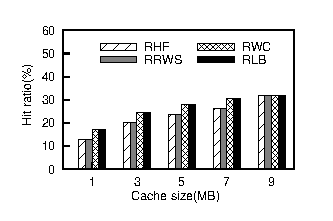
\includegraphics
   [height=3.5cm]{figure/aalborgHitVsCacheSize.eps}}
   \subfigure[{\footnotesize Beijing}]
   {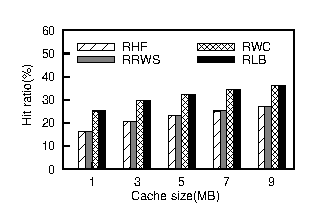
\includegraphics [height=3.5cm]{figure/beijingHitVsCacheSize.eps}}
   \subfigure[{\footnotesize Singapore}]
   {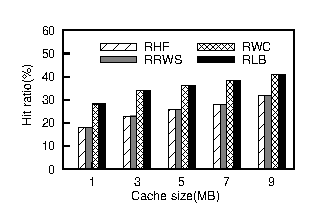
\includegraphics [height=3.5cm]{figure/singaporeHitVsCacheSize.eps}}
 \caption{Hit ratios of refreshment strategies.}
 \label{fig:comparison-hit}
\end{figure}


Next we test the refreshment time of these four replacement strategies along with various cache sizes on three data sets.
The refreshment time includes three parts: the time of detecting affected paths, the time of computing shortest paths by the server, and the time of selecting new paths into the cache. For RWC, the time of detecting affected paths is zero.
The experimental result (rf. Figure~\ref{fig:comparison-overall-time}) on each data set is the average of 50 instances.
The performance on three data sets is consistent; each method displays similar trends on three data sets.
RWC spends the most refreshment time, and the time increases as the cache size increases. It can be predicted that the disadvantage of RWC in refreshment time will amplify more if more shortest paths are queried, since RWC takes a lot of time to computing shortest paths every time the cache is emptied.
RLB, RHF, and RRWS spend similar time.
Precisely, RLB has the shortest refreshment time.
This is consistent with our analysis in Section~\ref{sec:strategies}.
 \begin{figure}[htbp]
\centering
   \subfigure[{\footnotesize Aalborg}]
   {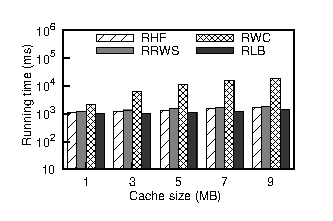
\includegraphics
   [height=3.5cm]{figure/A-size-method-time.eps}}
   \subfigure[{\footnotesize Beijing}]
   {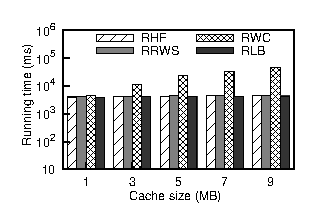
\includegraphics [height=3.5cm]{figure/A-size-method-time-beijing.eps}}
   \subfigure[{\footnotesize Singapore}]
   {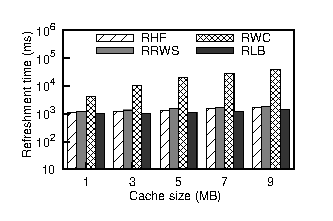
\includegraphics [height=3.5cm]{figure/SinggporeCache-size-time.eps}}
   \caption{Refreshment time of refreshment strategies.}
   \label{fig:comparison-overall-time}
\end{figure}

From the above experiments, we can see that RLB has the best running time and hit ratio. Hence, in the real applications, RLB is suggested to be used.



